%!TEX TS-program = pdflatex
%!TEX encoding = UTF-8 Unicode
%!TeX spellcheck = it_IT
%!TEX root = ../tesi.tex
%
\chapter{\textit{Obstacle Shadowing Model}}
\section{Network Simulator 3}
Network Simulator 3 (ns-3)~\cite{ns3Website} è un simulatore a eventi discreti utilizzato principalmente in ambito accademico e di ricerca,
scritto in \Cpp e Python; è un software libero distribuito sotto licenza GNU GPLv2.
Creato nel 2006 da un gruppo coordinato da Tom Henderson, George Riley, Sally Floyd e Sumit Roy con lo scopo
di ovviare ad alcune grosse limitazioni della precedente versione (ns-2), come ad esempio la necessità di utilizzare
un linguaggio di \textit{scripting} dedicato per modellare le simulazioni o una maggiore scalabilità~\cite{Henderson:2006:NPG:1190455.1190468}.
Attualmente è l'unica versione della serie a essere sviluppata.
È d'obbligo menzionare che, sebbene tutte le versione siano state scritte in \Cpp, questa non è retrocompatibile con le precedenti.
%
\subsection{Concetti chiave}
Alcuni concetti chiave:
\begin{itemize}
	\item In ns-3, l'unità elementare è chiamata \textit{nodo}: questa fornisce i metodi per gestire i dispositivi nelle simulazioni.
	\item Sui nodi girano delle \textit{applicazioni}: queste eseguono delle azioni per giungere a un obbiettivo.
				Per esempio, le applicazioni \textsf{UdpEchoClientApplication} e \textsf{UdpEchoServerApplication} compongono
				un'aplicazione client/server per gestire e scambiare pacchetti nella rete.
	\item Le comunicazioni fra i nodi avvengono tramite degli speciali \textit{canali};
				i canali modellano diversi concetti, dai più semplici come un collegamento su cavo a quelli più complessi
				come uno switch Ethernet.
				Il canale \textsf{CsmaChannel}, ad esempio, modella un mezzo tramissivo con accesso CSMA.
	\item Sui nodi si installano dei \textit{dispositivi di rete} che permettono la comunicazione fra questi attraverso i canali.
				Un nodo può essere connesso a più canali attraverso diversi dispositivi di rete.
				Per utilizzare il canale \textsf{CsmaChannel} è presente il dispositivo \textsf{CsmaNetDevice}.
\end{itemize}
%
\section{Il modello matematico}
Gli autori di~\cite{Carpenter:2015:OMI:2756509.2756512} riprendono il modello introdotto da Christoph Sommer et al.\ in~\cite{5720204},
nel quale la perdita di segnale dovuta a ostacoli $L_{s,o}$ dipende dall'attenuazione causata dai bordi dell'ostacolo (\textit{per-wall attenuation})
e quella derivante dalla superficie interna (\textit{per-meter attenuation}):
\begin{gather}\label{eq:osbtacle-model}
	L_{s,o} = \alpha n + \beta d_o
\end{gather}
Nella formula precedente, $n$ indica il numero di volte che il bordo dell'ostacolo viene intersecato dalla visuale (of LoS, da \textit{Line of sight}),
mentre $d_o$ è la distanza, in metri, attraversa all'interno dell'ostacolo.
Il parametro $\alpha$ rappresenta l'attenuazione per-metro espressa in decibels (dBm), invece
$\beta$ l'attenuazione per-metro, sempre in decibels (dB/m).

I due fattori di calibrazione permettono di rappresentare più tipologie di edificio.
I valori predefiniti di $\alpha = 9$ dBm e $\beta = 0,4$ dB/m sono buoni per la maggior parte delle applicazioni
anche se, naturalmente, non per tutte.
Riportando l'esempio in~\cite{5720204} di una casa in costruzione, il modello riesce a rappresentare le caratteristiche dell'attenuazione,
tuttavia i parametri sono distanti da quelli sopra indicati: $\alpha$ = 2.4 dBm and $\beta$ = 0.63 dB/m.
%
\begin{figure}[!h]
	\centering
	\begin{center}
		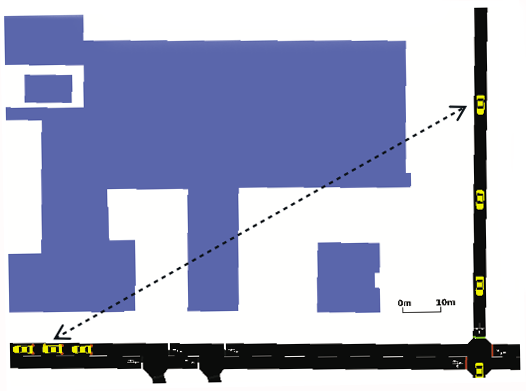
\includegraphics[width=.8\textwidth]{carpenter-1.png}
	\end{center}
	\label{fig:scenario-urbano-1}\caption{Esempio di scenario urbano.}
\end{figure}
%
Prendiamo l'esempio raffigurato in Figura~\ref{fig:scenario-urbano-1}, dove la linea fra i due veicoli interseca $n=6$ muri e una distanza interna di $d_o=32$m;
sostituendo i valori in~\ref{eq:osbtacle-model} si ottiene: $L_{s,o} = 9*6 + 0,4*32 = 66,8$dB.
Si evince come, con questa quantità di attenuazione, sia difficile che la trasmissione da un veicolo abbia abbastanza potenza per essere ricevuta dal secondo veicolo.
%
\section{L'implementazione}
Nel dettaglio, gli ostacoli sono rappresentati da poligoni bidimensionali che ne definiscono i bordi (spigoli).
Riprendendo l'esempio in Figura~\ref{fig:scenario-urbano-1}, la linea di visibilità (in questo caso \textit{obstructed-line-of-sight}, OLOS), fra i due veicoli potrebbe
intersecare diversi muri e percorrere una certa distanza internamente a uno o più edifici.
Il modello \textit{Obstacle Shadowing} conta il numero di intersezioni con gli spigoli dell'ostacolo, calcola la distanza percorsa internamente a esso e, utilizzando
il modello matematico visto in precedenza, restituisce l'attenuazione della trasmissione wireless fra i due veicoli.

Il tutto è implementato in ns-3 tramite tre classi: \textsf{Obstacle} contiente la rappresentazione geometrica dell'ostacolo, utilizzando le Computational Geometry Algorithms Library (CGAL),
come anche i parametri dell'attenuazione per-metro e per-muro.
\textsf{Topology} legge i dati degli edifici da un file specifico, generato dall'utility Polyconvert del software SUMO (Simulator for Urban Mobility)~\cite{sumoWebsite}
a partire dalle informazioni ottenute da OpenStreetMap (OSM)~\cite{osmWebsite}.
L'oggetto \textsf{Topology} così creato è poi utilizzato per determinare la perdita di segnale fra due punti (e.g. veicoli), utilizzando l'algoritmo illustrato
in Figura~\ref{fig:algoritmo-getobstucteddistancebetween}.
%
\begin{algorithm}[!h]
\caption{Algoritmo per determinare il numero di intersezioni con i bordi dell'ostacolo e la distanza interna percorsa fra due punti.}\label{fig:algoritmo-getobstucteddistancebetween}
\begin{algorithmic}[1]
	\Procedure{GetObstuctedDistanceBetween}{$p_1, p_2, B$}
	\BState{}\emph{Input}: $p_1, p_2$: posizione dei due veicoli; $B$: partizione binaria dello spazio (BSP) di ostacoli.
	\BState{}\emph{Output}: Distanza interna percorsa, $m_o$, e il numero di intersezioni con i bordi, $n$.
	\State{$m_o \gets 0;\; n \gets 0$}
	\TextState{Inizializza la portata massima $r$: distanza dal punto $p_1$ o $p_2$ al centro di un ostacolo, utilizzata per filtrare il sottoinsieme di ostacoli sufficientemente vicini.}
	\TextState{Crea un riquadro di delimitazione $b$ per $p_1$ e $p_2$ ed estendila di $r$ in tutte le direzioni.}
	\TextState{Calcola l'insieme di potenziali ostacoli $O$ da quelli all'interno di $b$ in $B$.}
	\ForEach{ostacolo $o \in O$}
		\If{(distance($p_1$, o.center) $< r$) OR (distance($p_2$, o.center) $< r$)}
			\ForEach{spigolo $e \in o$}
				\If{$s$ interseca un raggio da $p_1$ a $p_2$}
					\State{$n \gets n+1$}
					\TextState{Salva la distanza minima e massima da $\{ p_1, p_2\}$ al punto d'intersezione.}
				\EndIf{}
				\TextState{$m_o \gets m_o+$ differenza fra i valori min e max calcolati al passo precedente.}
			\EndFor{}
		\EndIf{}
	\EndFor{}
	\Return{$m_o$ e $n$}
	\EndProcedure{}
\end{algorithmic}
\end{algorithm}
%
\section{Utilizzo}
Per impostare una simulazione che utilizzi sono necessari alcuni passaggi, come illustrato in Figura  
